\documentclass[aps,prd,onecolumn,notitlepage,nofootinbib,superscriptaddress,altaffilletter,floatfix]{revtex4-1}

%\documentclass[twocolumn,superscriptaddress,showpacs,preprintnumbers,amsmath,amssymb]{revtex4}
%\documentclass[,showpacs,preprintnumbers,amsmath,amssymb]{revtex4}

%\bibliographystyle{unsrt}
%ieeetr
\usepackage{graphicx}% Include figure files
\usepackage{float}
\usepackage{amssymb}
\usepackage{amsmath}
\usepackage{longtable}
\usepackage{color}
\usepackage{hyperref}

% Bibliography style
%%\bibliographystyle{abbrvnat}
\bibliographystyle{apsrev}

\usepackage{soul}
\newcommand{\repr}[1]{{\color{red}[#1]}}
\newcommand{\strike}[1]{{\color{red}\st{#1}}}

\newcommand{\tStart}{t_0}
\newcommand{\tEvent}{t_{\mathrm{event}}}
\newcommand{\tMerger}{t_{\mathrm{M}}}
\newcommand{\freq}{f_0}

\newcommand{\parA}{{\mathcal A}}
\newcommand{\As}{\parA_{\mathrm{s}}}
\newcommand{\Ac}{\parA_{\mathrm{c}}}

\newcommand{\xs}{x_{\mathrm{s}}}
\newcommand{\xc}{x_{\mathrm{c}}}
\newcommand{\xvec}{\vec{x}}

\newcommand{\hs}{h_\mathrm{s}}
\newcommand{\hc}{h_\mathrm{c}}
\newcommand{\hexp}{h_{\mathrm{exp}}}
\newcommand{\Is}{I_{\mathrm{s}}}
\newcommand{\Ic}{I_{\mathrm{c}}}
\newcommand{\Isc}{I_{\mathrm{sc}}}
\newcommand{\M}{\mathcal{M}}
\newcommand{\Mss}{\M_{\mathrm{ss}}}
\newcommand{\Mcc}{\M_{\mathrm{cc}}}
\newcommand{\Msc}{\M_{\mathrm{sc}}}

\newcommand{\Dt}{\Delta t}
\newcommand{\scalar}[2]{\left\langle #1\middle|#2\right\rangle}
\newcommand{\Hyp}{\mathcal{H}}
\newcommand{\HypG}{\Hyp_{\mathrm{G}}}
\newcommand{\HypS}{\Hyp_{\mathrm{S}}}
\newcommand{\prob}[2]{P\left(#1\middle|#2\right)}
\newcommand{\FT}[1]{\widetilde{#1}}
\newcommand{\parE}{\lambda}
\newcommand{\BSG}{B_{\mathrm{S/G}}}
\newcommand{\Lr}{\mathcal{L}}
\newcommand{\Ord}[1]{\mathcal{O}\left(#1\right)}

\newcommand{\MP}{{\mathrm{MP}}}

\newcommand{\Sn}{\mathcal{S}}
\newcommand{\SX}{S_X}
\newcommand{\Ndet}{N_{\mathrm{det}}}
\newcommand{\sig}{{\mathrm{sig}}}
\newcommand{\Gam}{\gamma}
\newcommand{\eye}{\mathbb{I}}
\newcommand{\Fab}{F}
\newcommand{\F}{\mathcal{F}}
\newcommand{\trace}[1]{\mathrm{tr}#1}
%% ---------- Units ----------
\newcommand{\ms}{\mathrm{ms}}
\newcommand{\Hz}{\mathrm{Hz}}
\renewcommand{\sec}{\mathrm{s}}
%%% Local Variables:
%%% mode: latex
%%% TeX-master: t
%%% End:

\input{git_tag.tex}

\newcommand{\dcc}{LIGO-T1500618-v3++}

\begin{document}

\title{Bayesian QNM search on GW150914}

%% \title{Template-based investigations to study the parameter-space metric for known continuous
%% wave sources in binary systems}

\author{Reinhard Prix}
\altaffiliation{Reinhard.Prix@ligo.org}
\affiliation{Max-Planck-Institut f\"ur Gravitationsphysik, Albert-Einstein-Institut, D-30167 Hannover, Germany}
\date{\commitDATE; \commitIDshort-\commitSTATUS; \href{https://dcc.ligo.org/LIGO-T1500618}{\dcc}}
%\parbox[c]{1em}{\textcolor{red}{DRAFT}}


\begin{abstract}
  We quantify the evidence for and estimate the parameters of QNM 'ringdown' in the GW150914 event.
  This is done by Bayesian hypothesis testing and parameter estimation using a QNM ringdown model
  $s(t\ge\tStart) = A\,e^{-\frac{t-\tStart}{\tau}}\cos\left(2\pi \freq (t-\tStart) + \phi_0\right)$ with unknown amplitude $A$, initial phase $\phi_0$,
  frequency $\freq$ and decay time $\tau$, as a function of the QNM start-time $\tStart$.
  Using a Gaussian-isotropic prior on $\{\As=-A\sin\phi_0,\,\Ac=A\cos\phi_0\}$ we can approximate the Bayes factor by analytically marginalizing over
  $\{A,\phi_0\}$, leaving an explicit template search over $\{\freq,\,\tau\}$. We search the range $f\in[200,\,300]\,\Hz$ and $\tau \in [0.5, 20]\,\ms$
  assuming a uniform prior.

  \textbf{Note}: This version (v3++) includes a bugfix in octapps that results in slightly different numerical results, but which qualitatively agree with previous ones (v3+).
\end{abstract}

%%\pacs{04.80.Nn, 95.55.Ym, 95.75.-z, 97.60.Gb, 07.05.Kf}% PACS, the Physics and Astronomy
\maketitle

%%%%%%%%%%%%%%%%%%%%%%%%%%%%%%%%%%%%%%%%%%%%%%%%%%%%%%%%%%%%%%%%%%%%%%%%%%%%%%%%%%%%%%%
\section{Introduction}
\label{Intro}
%%%%%%%%%%%%%%%%%%%%%%%%%%%%%%%%%%%%%%%%%%%%%%%%%%%%%%%%%%%%%%%%%%%%%%%%%%%%%%%%%%%%%%%

Signal model: damped sinusoid starting at $\tStart$:
\begin{align}
  \label{eq:1}
  s(t;\,A, \phi_0\,, \tStart, \tau, \freq) &= A\,w(t-\tStart,\,\tau)\,\cos\left(2\pi\,\freq\,(t-\tStart) + \phi_0\right)\,,\\
  w(t, \tau) &=
  \begin{cases}
    \exp\left( -\frac{t}{\tau} \right) & \text{if } t \ge 0\,\\
    0  & \text{if } t < 0
  \end{cases}
\end{align}
Rewrite waveform in terms of two unknown amplitudes $\As = -A\,\sin\phi_0,\,\Ac = A\,\cos\phi_0$ in ``JKS'' factorization
\cite{bretthorst1988:_bayesian_spectrum,jks98:_data}:
\begin{equation}
  \label{eq:2}
  s(t; \parmsAll) = \As \, \hs(t;\parmsEvol) + \Ac\,\hc(t;\parmsEvol)\,,
\end{equation}
with \emph{basis functions}
\begin{align}
  \label{eq:14}
  \hs(t;\parmsEvol) &\equiv w(t-\tStart,\tau)\,\sin(2\pi \,\freq\,(t-\tStart))\,,\\
  \hc(t;\parmsEvol) &\equiv w(t-\tStart,\tau)\,\cos(2\pi \,\freq\,(t-\tStart))\,,
\end{align}
and the set of signal parameters separating into ``amplitude parameters'' $\Avec$ and ``evolution parameters'' $\parmsEvol$:
\begin{equation}
  \label{eq:11}
  \parmsAll \equiv \{\Avec, \parmsEvol\}\,,
  \quad \Avec \equiv \left(\As,\Ac\right)\,,
  \quad \parmsEvol \equiv \{\tStart,\tau, \freq\}\,.
\end{equation}
The likelihoods for Gaussian (colored) noise $\HypG$ and the ringdown model $\HypS$ are
\begin{align}
  \label{eq:4}
  \prob{x}{\HypG} &= c\,e^{-\frac{1}{2}\scalar{x}{x}}\,,\\
  \prob{x}{\HypS,\parmsAll} &= c\,e^{-\frac{1}{2}\scalar{x-s(\parmsAll)}{x-s(\parmsAll)}}\,,
\end{align}
with the multi-detector scalar product (over detector index $X$) defined as
\begin{equation}
  \label{eq:5}
  \scalar{x}{y}\equiv \sum_{X} \scalar{x^X}{y^X} = \sum_X 2\int_{-\infty}^{\infty} \frac{\FT{x}^X(f)\,\FT{y}^{*X}(f)}{S_X(f)}\,df\,,
\end{equation}
with the per-detector single-sided noise PSD $S_X(f)$ (which results in the prefactor of '2').
The (marginal) likelihood for the signal model can be expressed as
\begin{equation}
  \label{eq:6}
  \prob{x}{\HypS} = \int \prob{x}{\HypS,\parmsAll}\,\prob{\parmsAll}{\HypS}\,d\parmsAll\,,
\end{equation}
and the corresponding Bayes factor (or marginal likelihood ratio)
\begin{equation}
  \label{eq:7}
  \BSG(x) \equiv \frac{\prob{x}{\HypS}}{\prob{x}{\HypG}} = \int \Lr(x;\parmsAll)\,\prob{\parmsAll}{\HypS}\,d\parmsAll\,,
\end{equation}
with the likelihood-ratio \emph{function}
\begin{equation}
  \label{eq:8}
  \Lr(x;\parmsAll) \equiv \frac{\prob{x}{\HypS,\parmsAll}}{\prob{x}{\HypG}} = \exp\left(\scalar{x}{s} - \frac{1}{2}\scalar{s}{s}\right)\,.
\end{equation}
We can further introduce a partially-marginalized (over unknown amplitude parameters $\Avec$) Bayes factor $\BSG(x;\parmsEvol)$ as
\begin{align}
  \BSG(x) &= \int \Lr(x;\parmsAll)\,\prob{\parmsAll}{\HypS}\,d\parmsAll \notag\\
          &= \int \Lr(x;\Avec,\parmsEvol)\,\prob{\Avec}{\parmsEvol,\HypS}\,\prob{\parmsEvol}{\HypS}\,d^2\A\,d\parmsEvol \notag\\
          &= \int \BSG(x;\parmsEvol) \,\prob{\parmsEvol}{\HypS}\,d\parmsEvol\,,   \label{eq:23a}\\
  \BSG(x;\parmsEvol) &\equiv \int \Lr(x;\A,\parmsEvol)\prob{\A}{\parmsEvol,\HypS}\,d^2\A\,.  \label{eq:23b}
\end{align}

\section{Computing the Bayes factor $\BSG$}
\label{sec:comp-bayes-fact}

\subsection{Expressing the SNR$^2$: $\scalar{s}{s}$}
\label{sec:computing-scalarss}

We assume the data $x^X(t)$ from the different detectors has been time-shifted and corrected for antenna-pattern effects, in such a way that the
expected signal $s(t)$ would be identical in all data streams, so we can assume the templates to be independent of detector, and write
\begin{align}
  \label{eq:15}
  \scalar{s}{s} &= \sum_X 2\int_{-\infty}^{\infty} \frac{\left| \FT{s}(f) \right|^2}{\SX(f)}\,df\\
  &= 2\Ndet\,\int \frac{\left| \FT{s}(f) \right|^2}{\Sn(f)}\,df\,,
\end{align}
where the multi-detector noise floor $\Sn(f)$ is defined as the harmonic mean
\begin{equation}
  \label{eq:26}
  \Sn^{-1}(f) \equiv \frac{1}{\Ndet}\sum_X S_X^{-1}(f)\,.
\end{equation}
Using the factorization of Eq.~\eqref{eq:2}, which in frequency domain yields
\begin{equation}
  \label{eq:34}
  \FT{s}(f;\parmsAll) = \As\,\FT{\hs}(f;\parmsEvol) + \Ac\,\FT{\hc}(f;\parmsEvol)\,,
\end{equation}
we can further write this as
\begin{equation}
  \label{eq:36}
  \scalar{s}{s} = \Avec \cdot \M(\parmsEvol) \cdot \Avec\,,
\end{equation}
with
\begin{align}
  \label{eq:35}
  \M(\parmsEvol) &\equiv
  2\Ndet \begin{pmatrix}
    \Is  & \Isc \\
    \Isc  & \Ic\\
  \end{pmatrix}\,,\\
  \Is(\parmsEvol) &= 2 \int_{0}^{\infty} \frac{|\FT{\hs}(f)|^2}{\Sn(f)}\,df \,,\\
  \Ic(\parmsEvol) &= 2 \int_{0}^{\infty} \frac{|\FT{\hc}(f)|^2}{\Sn(f)}\,df \,,\\
  \Isc(\parmsEvol)&= 2 \int_{0}^{\infty} \frac{\Re[\FT{\hs}(f)\,\FT{\hc}^{*}\!\!(f)]}{\Sn(f)}\,df \,.
\end{align}
The Fourier transforms $\FT{\hs},\FT{\hc}$ of the signal basis functions can be computed analytically
\begin{align}
  \label{eq:37}
  \FT{\hs}(f;\parmsEvol) &= \tau\,\frac{2\pi\freq\,\tau}{1 + i\,4\pi\,f\,\tau -  4\pi^2(f^2 - \freq^2)\tau^2} \, e^{-i2\pi f\tStart} \,,\\
  \FT{\hc}(f;\parmsEvol) &= \tau\,\frac{1 + i\,2\pi\,f\,\tau}{1 + i\,4\pi\,f\,\tau - 4\pi^2(f^2 - \freq^2)\tau^2} \, e^{-i2\pi f\tStart} \,.
\end{align}


\subsection{Expressing the ``matched filter'' $\scalar{x}{s(\parmsAll)}$}
\label{sec:computing-scalarxs}

Note that in the scalar product involving the data $x^X$ (assume time-shifted and antenna-pattern corrected) we can conveniently absorb the
frequency-dependend noise-floors $S_X(f)$ by \emph{over-whitening} the data, i.e.\ we define
\begin{equation}
  \label{eq:12}
  \FT{y}^X \equiv \frac{\FT{x}^X(f)}{S_X(f)}\,,\quad
  \FT{y} \equiv \sum_X \FT{y}^X\,.
\end{equation}
Here we define $t$ to the arrival time in the 'H1' detector.
We apply a detector-specific time-delay of adding $7\,\ms$ to L1 arrival time in the case of GW150914) and
antenna-pattern corrections (a factor of $-1$ of L1 wrt H1) to the \emph{data} $y^X(t)$, such that we can assume the putative signal waveform in the
data to be in phase and of (approximately) same amplitude and phase. This means that we can assume a detector-independent template $s^X(t) = s(t)$,
which allows us to write the scalar product in time-domain form
\begin{align}
  \label{eq:13}
  \scalar{x}{s(\parmsAll)} &= \sum_X 2\int_{-\infty}^{\infty} \FT{y}^X(f)\,\FT{s}^{*X}(f)\,df \\
  &= 2\int_{-\infty}^{\infty} \FT{y}(f)\,\FT{s}^{*}(f)\,df \\
  &=  2\int_{\tStart}^{\tStart + T} y(t)\,s(t)\,dt\,,
\end{align}
where $y(t)$ is the overwhitened summed-IFO timeseries, i.e.\ the inverse Fourier-transform of $\FT{y}(f)$, and
where $T \gg \tau$ is some duration long enough so that $s(\tStart+T)\approx0$, e.g.\ $T=5\tau$.

Using Eq.~\eqref{eq:2} we can further write
\begin{equation}
  \label{eq:9}
  \scalar{x}{s(\parmsAll)} = \Avec\cdot\xvec(\parmsEvol) = \As\,\xs(\parmsEvol) + \Ac\,\xc(\parmsEvol)\,,
\end{equation}
with
\begin{align}
  \label{eq:10}
  \xs(\parmsEvol) &\equiv 2\int_{\tStart}^{\tStart+T} y(t)\,\hs(t;\parmsEvol)\,dt\,,\\
  \xc(\parmsEvol) &\equiv 2\int_{\tStart}^{\tStart+T} y(t)\,\hc(t;\parmsEvol)\,dt\,.
\end{align}
Note that it will be convenient to write
\begin{equation}
  \label{eq:38}
  \hexp \equiv \hc(t;\parmsEvol) - i\,\hs(t;\parmsEvol) = e^{-\Dt/\tau}\,e^{-i\,2\pi\,\freq\,\Dt} = e^{-\Dt \,\varpi}\,,
\end{equation}
with $\Dt \equiv t - \tStart$ and complex frequency $\varpi$ defined as
\begin{equation}
  \label{eq:27}
  \varpi \equiv \frac{1}{\tau} + i\,2\pi \freq\,,
\end{equation}
and so we obtain the complex matched-filter as
\begin{equation}
  \label{eq:16}
  \Fab \equiv \xc - i\,\xs = 2 \int_{0}^{T} y(\tStart+\Dt)\,e^{-\Dt \,\varpi}\,d\Dt\,,
\end{equation}
which is the Laplace transform of the over-whitened data $y(t)$.

\subsection{Marginalizing over unknown amplitudes $\{\As,\Ac\}$}
\label{sec:marg-over-unkn}

Combining these expressions in the likelihood-ratio function of Eq.~\eqref{eq:8}, we can write this as
\begin{align}
  \label{eq:21}
  \ln \Lr(x;\parmsAll) &= \scalar{x}{s} - \frac{1}{2}\scalar{s}{s}\\
  &= -\frac{1}{2}\,\Avec\cdot\M\cdot\Avec + \Avec\cdot\xvec\,,
\end{align}
i.e.\ a 2-dimensional Gaussian in $\{\As,\Ac\}$ with covariance matrix $\M^{-1}$.
This can be marginalized analytically to yield $\BSG(x;\parmsEvol)$ in Eq.~\eqref{eq:23a} for a suitable choice of prior
$\prob{\Avec}{\parmsEvol,\HypS}$.

First we assume that the amplitude prior is \emph{logically} independent of the evolution parameters $\parmsEvol$, which simply expresses ignorance about a
possible dependence, not a claim about \emph{physical} independence \cite{jaynes:_logic_of_science},
i.e.\ $\prob{\Avec}{\parmsEvol,\HypS} = \prob{\Avec}{\HypS}$

Further we use a simple isotropic Gaussian amplitude prior, which expresses ignorance about the initial phase $\phi_0$, and posits an (unknown)
characteristic scale $H$ for the amplitude $A$, namely
\begin{equation}
  \label{eq:22}
  \prob{\Avec}{\HypS,H} = \frac{1}{2\pi\,H^2}\,e^{-\frac{1}{2}{\Avec\cdot\Avec}/H^2}\,\,,
\end{equation}
which implies a prior on the amplitude $A$ (marginalized over $\phi_0$):
\begin{equation}
  \label{eq:28}
  \prob{A}{\HypS, H} = \frac{A}{H^2}\,e^{-\frac{A^2}{2H^2}}\,.
\end{equation}
Using this Gaussian amplitude prior we find the $H$-dependent Bayes factor:
\begin{align}
  \label{eq:29}
  \BSG(x;\parmsEvol,H) &\equiv \frac{\prob{x}{\HypS,\parmsEvol,H}}{\prob{x}{\HypG}}\\
  &=\frac{1}{2\pi H^2}\int e^{-\frac{1}{2}\,\Avec\cdot\Gam^{-1}\cdot\Avec + \Avec\cdot\xvec}\,d^2\A\\
  &= \frac{\sqrt{\det\Gam}}{H^2}\, e^{\frac{1}{2}\,\xvec\cdot\Gam\cdot\xvec}
\end{align}
with
\begin{equation}
  \label{eq:25}
  \Gam^{-1}(\parmsEvol) \equiv \M + H^{-2}\,\eye =
  \begin{pmatrix}
    \Is + H^{-2} & \Isc \\
    \Isc        & \Ic + H^{-2}\,.
  \end{pmatrix}\,,
\end{equation}
and determinant
\begin{align}
  \label{eq:39}
  \det\Gam^{-1} &= \left(\Is + H^{-2}\right)\left(\Ic+H^{-2}\right) - \Isc^2\\
  &=\det\M + H^{-2}\,\trace{\M} + H^{-4}\,,
\end{align}
inverse
\begin{equation}
  \label{eq:41}
  \Gam(\parmsEvol) = \frac{1}{\det\Gam^{-1}}
  \begin{pmatrix}
    \Ic + H^{-2} & -\Isc \\
    -\Isc        & \Is + H^{-2}
  \end{pmatrix}\,,
\end{equation}
and
\begin{equation}
  \label{eq:40}
  \frac{\sqrt{\det\Gam}}{H^2} = \left[H^4\,\det\M + H^2\,\trace{\M} + 1\right]^{-1/2}\,.
\end{equation}

We note that in the limit $H\rightarrow0$ we have $\Gam^{-1}\rightarrow H^{-2}\eye$, so $\Gam\rightarrow0$, and
$\sqrt{\det\Gam}/H^2\rightarrow 1$, therefore $\BSG\rightarrow 1$.
The signal hypothesis becomes indistinguishable from the noise hypothesis if signal amplitudes are assumed to be vanishingly small.
In the opposite limit of $H\gg 1$, we find $\Gam\rightarrow\M^{-1}$, and $\sqrt{\det\Gam}/H^2\rightarrow 1/(H^2\sqrt{\det\M})$, which is equivalent to
the ``$\F$-statistic'' for finite $H$, but $\BSG\rightarrow 0$ for $H\rightarrow \infty$, as the prior volume gets increasingly thinly spread out,
resulting in an ``Occam factor'' effect disfavoring the signal hypothesis.

\subsubsection{Marginalizing unknown scale $H$}
\label{sec:marg-unkn-scale}

The most robust way to deal with the unknown scale parameter $H$ is to marginalize this out using a Jeffreys prior $\propto 1/H$. Given that we
\emph{roughly} know the scale of $H$ to fall somewhere in $H\in[2,10]\times10^{-22}$, we can simply discretize the corresponding marginalization
integrals on a few points ${H_i}$, allowing us to normalize this discrete ``hyper-prior'' as
\begin{equation}
  \label{eq:44}
  \prob{H_i}{\HypS} = c\,\frac{1}{H_i},,\quad\text{with}\quad c^{-1} = \sum_i H_i^{-1}\,.
\end{equation}
We can therefore estimate the unknown $H$ parameter from the data via Eq.~\eqref{eq:29}, namely
\begin{align}
  \label{eq:45}
  \prob{H}{x} &= \int \prob{\parmsEvol,H}{x,\HypS}\,d\parmsEvol\\
  &= \left[\int \prob{x}{\HypS,\parmsEvol,H}\,\prob{\parmsEvol}{\HypS}\,d\parmsEvol\right]\,\prob{H}{\HypS}\\
  &\propto \BSG(x;H)\,\prob{H}{\HypS} \\
  &= c\,\frac{1}{H_i}\,\BSG(x;H_i)\,.
\end{align}
Furthermore, we can compute the $H$-independent Bayes factor and posterior by marginalizing over $H$ via
\begin{align}
  \label{eq:46}
  \prob{\parmsEvol}{\HypS,x} &\propto \BSG(x;\parmsEvol)\\
  &=\int \BSG(x;\parmsEvol,H)\prob{H}{\HypS}\,dH\\
  &= c\,\sum_i \frac{1}{H_i} \, \BSG(x;\parmsEvol,H_i)\,.
\end{align}

\section{Parameter estimation}
\label{sec:parameter-estimation}

The posterior is
\begin{align}
  \prob{\parmsAll}{x,\HypS} &\propto \prob{x}{\HypS,\parmsAll}\,\prob{\parmsAll}{\HypS} \notag\\
    &\propto \Lr(x;\parmsAll)\,\prob{\A}{\HypS}\,\prob{\parmsEvol}{\HypS} \notag\\
    &\propto \exp\left[-\frac{1}{2}\, \Avec\cdot\Gam^{-1}\cdot\Avec + \Avec\cdot\xvec\right]\,\prob{\parmsEvol}{\HypS}\,.  \label{eq:30}
\end{align}
where in the first line we have dropped the normalization $1/\prob{x}{\HypS}$, and in the second line we dropped $\prob{x}{\HypG}$, as both are
independent of $\parmsAll$.
After marginalization over $\{\As,\Ac\}$ we recover again the Bayes factor $\BSG(x;\parmsEvol)$ of \eqref{eq:29}, i.e.
\begin{equation}
  \label{eq:32}
  \prob{\parmsEvol}{x,\HypS} \propto \BSG(x;\parmsEvol)\,.
\end{equation}

Finding the maximum-posterior estimates (MPE) for $\As,\Ac$ at fixed $\parmsEvol$ from \eqref{eq:30} yields
\begin{equation}
  \label{eq:31}
  \Avec' = \Gam(\parmsEvol)\cdot\xvec\,.
\end{equation}
Note that this depends on the unknown scale parameter $H$, but we will simplify this by using the MPE estimator for $H$ from Eq.~\eqref{eq:45}, i.e.\
$H_{MPE}$ that maximizes  $\BSG(x;H) / H$.
We will further evaluate this at the MPE values found for $\parmsEvol$ in the Bayes-factor search using \eqref{eq:32}.
From these we can obtain $A' = \sqrt{\As^2+\Ac^2}$ and $\phi_0' = - \tan^{-1}\left(\frac{\As}{\Ac}\right)$.

From this can can also estimate an ``SNR'' in the MPE template, by substituting the MPE amplitude parameters into the SNR expression
Eq.~\eqref{eq:36}, i.e.\
\begin{equation}
  \label{eq:20}
  \rho_0^2 = \Avec'\M\Avec'\,.
\end{equation}

\newpage
\section{QNM search applied to GW150914}
\label{sec:qnm-search-applied}

\subsection{Prior choices}
\label{sec:prior-choices}

Isotropic 2D Gaussian amplitude prior \eqref{eq:22} on $\{\As,\Ac\}$ with characteristic amplitudes $H = [2,4,6]\times10^{-22}$, which corresponds to
isotropic prior in $\phi_0$ and an $A$-prior of \eqref{eq:28}, as shown here:\\
\parbox{\textwidth}{
  \centering
  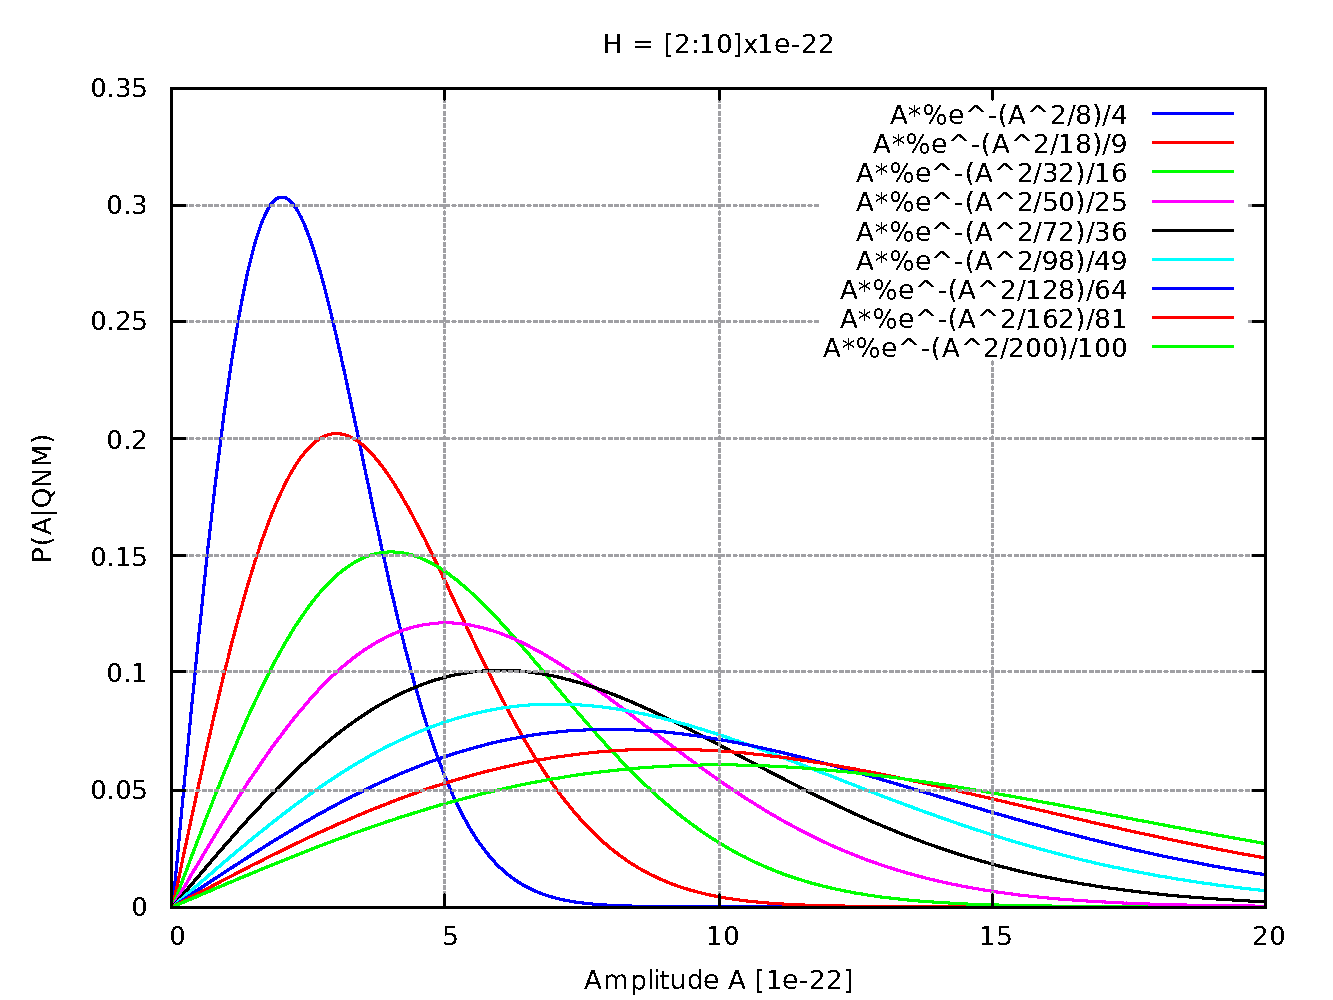
\includegraphics[width=0.4\textwidth]{prior_A.pdf}
}
%%\caption{Amplitude $A$ prior with characteristic scale $H=4\times10^{-22}$}

\subsection{Data preparation}
\label{sec:data-preparation}

Band-passed data in (i) $[10,\,2000]\,\Hz$ (using tukey(0.1) windowing) on a 1800s Fourier-transform containing the GPS time
$\tEvent = 1126259462\,$s.
From this we extracted a $T=8\,$s timeseries $x^X(t)$ centered on the event GPS time $\tEvent$.
Time-shifted L1 data by (delaying it by $+7\,\ms$) and multiplied it by $(-1)$ to account for the inverse detector response.
We estimate the (single-sided) PSD $S_X$ by a standard welch method using 8s windows over the 1800s SFT data.

The resulting original spectrum (top row), rms-whitened spectrum (middle row) and over-whitened spectrum (bottom row) are shown in the following
plots, for H1 and L1, respectively.

\includegraphics[width=0.5\textwidth]{{../extractTS-Results/H-1_H1_1800SFT_ER8-C01-1126257832-1800-freq10Hz-2000Hz-fSamp4000Hz-GPS1126259462s+-4s-psd_v2-lineCleaningOff-spectrum}.pdf}
\includegraphics[width=0.5\textwidth]{{../extractTS-Results/L-1_L1_1800SFT_ER8-C01-1126258841-1800-freq10Hz-2000Hz-fSamp4000Hz-GPS1126259462s+-4s-psd_v2-lineCleaningOff-spectrum}.pdf}

\subsection{Numerical results}
\label{sec:numerical-results}

We search the $\{f,\tau\}$ range with uniform priors in $f\in[200,\,300]\,\Hz$ and $\tau\in[0.5,\,20]\,\ms$.
The following plots show snapshots of evidence and parameter-estimation at various fixed start-times $\tStart$, using a data frequency range of $[10,\,2000],\Hz$.
The offset from merger assumes a merger time $t_{\mathrm{merger}} = 1126259462.42285$ (in H1 arrival time), as taken from
\href{https://www.lsc-group.phys.uwm.edu/ligovirgo/cbcnote/TestingGR/O1/G184098/ringdown_presence}{Ian's wiki}. We show results for QNM start-times
$\tStart - t_{\mathrm{merger}} \in \{1,\,3,\,5,\,7\}\,\ms$ (always referring to H1 arrival times).

\newpage
\parbox{\textwidth}{
\includegraphics[width=0.9\textwidth]{{../Results/Results-160324-10h30-onSource-data10Hz-2000Hz-psd_v2-lineCleaningOff/Ringdown-GPS1126259462.423850s-f200Hz-300Hz-tau0.5ms-20.0ms-HJeffreys-psd_v2-lineCleaningOff}.pdf}\\
\includegraphics[width=0.9\textwidth]{{../Results/Results-160324-10h30-onSource-data10Hz-2000Hz-psd_v2-lineCleaningOff/Ringdown-GPS1126259462.425850s-f200Hz-300Hz-tau0.5ms-20.0ms-HJeffreys-psd_v2-lineCleaningOff}.pdf}
}

%%
\newpage
\vspace*{-2cm}\parbox{\textwidth}{
\includegraphics[width=0.9\textwidth]{{../Results/Results-160324-10h30-onSource-data10Hz-2000Hz-psd_v2-lineCleaningOff/Ringdown-GPS1126259462.427850s-f200Hz-300Hz-tau0.5ms-20.0ms-HJeffreys-psd_v2-lineCleaningOff}.pdf}\\
\includegraphics[width=0.9\textwidth]{{../Results/Results-160324-10h30-onSource-data10Hz-2000Hz-psd_v2-lineCleaningOff/Ringdown-GPS1126259462.429850s-f200Hz-300Hz-tau0.5ms-20.0ms-HJeffreys-psd_v2-lineCleaningOff}.pdf}
}

\newpage
\subsection{Summary plots}
\parbox{\textwidth}{
\includegraphics[width=0.9\textwidth]{{../Results/Results-160324-10h30-onSource-data10Hz-2000Hz-psd_v2-lineCleaningOff/Ringdown-GPS1126259462.423850s-f200Hz-300Hz-tau0.5ms-20.0ms-HJeffreys-psd_v2-lineCleaningOff-summary}.pdf}\\
\includegraphics[width=0.9\textwidth]{{../Results/Results-160324-10h30-onSource-data10Hz-2000Hz-psd_v2-lineCleaningOff/Ringdown-GPS1126259462.423850s-f200Hz-300Hz-tau0.5ms-20.0ms-HJeffreys-psd_v2-lineCleaningOff-contours}.pdf}
}

\newpage
\subsection{H-scale posteriors}

\includegraphics[width=0.9\textwidth]{{../Results/Results-160324-10h30-onSource-data10Hz-2000Hz-psd_v2-lineCleaningOff/Ringdown-GPS1126259462.423850s-f200Hz-300Hz-tau0.5ms-20.0ms-HJeffreys-psd_v2-lineCleaningOff-post_H}.pdf}\\
It seems the previous choice of a fixed scale $H = 4\times10^{-22}$ was not quite what the data favors, but also not too bad.


\newpage
\section{"Off Source"}

Analysing a data-segment that lies 10s past the event, going in steps of $50\,$ms for uncorrelated templates, 120 trials:\\
\parbox{\textwidth}{
\includegraphics[width=\textwidth]{{../Results/Results-160324-10h46-offSource-data10Hz-2000Hz-psd_v2-lineCleaningOff/Ringdown-GPS1126259469.422850s-f200Hz-300Hz-tau0.5ms-20.0ms-HJeffreys-psd_v2-lineCleaningOff-summary}.pdf}
\includegraphics[width=0.8\textwidth]{{../Results/Results-160324-10h46-offSource-data10Hz-2000Hz-psd_v2-lineCleaningOff/Ringdown-GPS1126259469.422850s-f200Hz-300Hz-tau0.5ms-20.0ms-HJeffreys-psd_v2-lineCleaningOff-hist}.pdf}
}

\newpage
\appendix

\section{Deprecated old way to compute $\scalar{s}{s}$: const noise floor + time-domain integration}
\label{sec:depr-first-way}

Given that aLIGO noise-curve is relatively ``white'' over a broad-band in the ``bucket'', and the signal $s(t)$ of Eq.~\eqref{eq:1} can still be
considered relatively ``narrow band'' ($\sim \pm 100\Hz$) with respect to this noise curve, we can approximate the signal-normalization integral as
\begin{align}
  \label{eq:17}
  \scalar{s}{s} &= \sum_X 2 \int_{-\infty}^{\infty} \frac{\FT{s}^X(f)\,\FT{s}^{*X}(f)}{S_X(f)}\,d f\\
  &\sim \sum_X \frac{2}{S_X(f')} \, \int_{0}^{\infty} s^2(t;\parmsAll)\,dt\\
  & = \frac{2\,\Ndet}{\Sn(f')} \,\int \left( \As^2\,\hs^2(t) + 2\As\Ac\,\hs\hc + \Ac^2\,\hc^2\right)\,d t\\
  & = \Avec \cdot \M \,\cdot\Avec\,,
\end{align}
with
\begin{equation}
  \label{eq:23}
  \M \equiv
  2\Ndet \begin{pmatrix}
    \Is  & \Isc \\
    \Isc  & \Ic\\
  \end{pmatrix}
\end{equation}
with
\begin{align}
  \label{eq:43}
  \Is  &\equiv \frac{1}{\Sn(f')}\int_0^\infty e^{-\frac{2t}{\tau}}\,\sin^2(2\pi f t)\,dt = \frac{1}{2\pi f}\int e^{-\frac{\varphi}{Q}} \sin^2\!\varphi\,d\varphi\\
  \Ic  &\equiv \int_0^\infty e^{-\frac{2t}{\tau}}\,\cos^2(2\pi f t)\,dt = \frac{1}{2\pi f}\int e^{-\frac{\varphi}{Q}} \cos^2\!\varphi\,d\varphi\\
  \Isc &\equiv \int_0^\infty e^{-\frac{2t}{\tau}}\,\sin(2\pi f t)\cos(2\pi f t)\,dt = \frac{1}{4\pi f}\int e^{-\frac{\varphi}{Q}} \sin2\varphi\,d\varphi\,,
\end{align}
where $f'$ is some (unknown) frequency within the effective frequency band around the central signal frequency $f$ (using mean-value theorem), and we
have used the assumption of identical signal model in both detectors (after time-shifting the data and correcting for antenna-pattern differences).

The respective integrals to compute are
\begin{align}
  \label{eq:18}
\end{align}
using the definitions
\begin{align}
  \label{eq:3}
  \varphi &\equiv 2\pi f \Dt\,,\\
  Q       &\equiv \pi f \tau\,.
\end{align}
Assuming only non-critically damped signals, i.e. $Q\gtrsim \Ord{\pi}$, these integrals can be approximated computed analytically as
\begin{align}
  \label{eq:19}
  \Is' &= \left. \frac{-1}{2\pi f}\frac{Q^2}{1 + 4Q^2}e^{-\frac{\varphi}{Q}}\left[ \sin2\varphi + 2Q + \frac{\sin^2\varphi}{Q}\right]\right|_0^\infty
  = \frac{2Q}{2\pi f}\,\frac{Q^2}{1+4Q^2}
  = \frac{\tau}{4 + Q^{-2}} \\
  & \stackrel{Q\gg1}{\approx} \frac{\tau}{4}\,,\\
  \Ic' &= \left. \frac{-1}{2\pi f}\frac{Q^2}{1 + 4Q^2}e^{-\frac{\varphi}{Q}}\left[ -\sin2\varphi + 2Q + \frac{\cos^2\varphi}{Q}\right]\right|_0^\infty
  = \frac{2Q + \frac{1}{Q}}{2\pi f}\,\frac{Q^2}{1+4Q^2} = \frac{\tau}{4}\,\left(\frac{2 + Q^{-2}}{2 + Q^{-2}/2}\right) \\
  & \stackrel{Q\gg1}{\approx} \frac{\tau}{4}\,,\\
  \Isc' &= \left. \frac{-1}{2\pi f}\frac{Q^2}{1 + 4Q^2}e^{-\frac{\varphi}{Q}}\left[ 2\cos^2\varphi - 1 + \frac{\sin2\varphi}{2Q}\right]\right|_0^\infty
  = \frac{1}{2\pi f}\,\frac{Q^2}{1+4Q^2} = \frac{\tau}{8Q\,(1 + Q^{-2}/4)}\\
  &\stackrel{Q\gg1}{\approx} \frac{1}{2Q}\,\Is \ll \Is \approx 0\,.
\end{align}
So $\Is \approx \Ic \approx \frac{\Ndet\tau}{2\Sn(f')}$ and $\Isc\approx 0$, and we obtain the approximate $\M$-matrix as
\begin{equation}
  \label{eq:42}
  \M \approx \frac{\Ndet\,\tau}{2\Sn(f')}\,\eye = \begin{pmatrix} I_0 & 0 \\ 0 & I_0 \end{pmatrix}\,.
\end{equation}
Note: in the QNM search we'll approximate $\Sn(f')$ in this expression by the arithmetic mean $\langle\Sn(f)\rangle_{f\pm\Delta f}$ around each
template frequency $f$. This fixed-SN high-Q limit was originally used in the \href{https://dcc.ligo.org/LIGO-G1600153-v1}{v1} of this search and
document, which was originally circulated.

\bibliography{RingdownSearch}

\end{document}

%%% Local Variables:
%%% ispell-local-dictionary: "american"
%%% fill-column: 150
%%% mode: latex
%%% mode: flyspell
%%% TeX-master: t
%%% End:
